% !TEX root = ../ComputationalOTFnT.tex

\chapter{Dynamic Formulations}
\label{c-dynamic}

This chapter presents the geodesic (also called dynamic) point of view of optimal transport when the cost is a squared geodesic distance. This describes the optimal transport between two measures as a curve in the space of measures minimizing a total length. The dynamic point of view offers an alternative and intuitive interpretation of optimal transport, which not only allows us to draw links with fluid dynamics but also results in an efficient numerical tool to compute OT in small dimensions when interpolating between two densities. The drawback of that approach is that it cannot scale to large-scale sparse measures and works only in low dimensions on regular domains (because one needs to grid the space) with a squared geodesic cost.

In this chapter, we use the notation $(\al_0,\al_1)$ in place of $(\al,\be)$ in agreement with the idea that we start at time $t=0$ from one measure to reach another one at time $t=1$.

%%%%%%%%%%%%%%%%%%%%%%%%%%%%%%%%%%%%%%%%%
\section{Continuous Formulation}

In the case $\X=\Y=\RR^d$, and $c(x,y)=\norm{x-y}^2$, the optimal transport distance $\Wass_2^2(\al,\be) = \MK_\c(\al,\be)$ as defined in~\eqref{eq-mk-generic} can be computed by looking for a minimal length path $(\al_t)_{t=0}^1$ between these two measures. 
%
This path is described by advecting the measure using a vector field $\speed_t$ defined at each instant. The vector field $\speed_t$ and the path $\alpha_t$ must satisfy the conservation of mass formula, resulting in 
\eql{\label{eq-cons-bb-ncvx}
	\pd{\al_t}{t} + \diverg(\al_t \speed_t) = 0
	\qandq 	
	\al_{t=0}=\al_0, 
	\al_{t=1}=\al_1,
}
where the equation above should be understood in the sense of distributions on $\RR^d$. The infinitesimal length of such a vector field is measured using the $L^2$ norm associated to the measure $\al_t$, that is defined as 
\eq{\norm{\speed_t}_{L^2(\al_t)} = \left( \int_{\RR^\dim} \norm{\speed_t(x)}^2 \d\al_t(x) \right)^{1/2}.} 
This definition leads to the following minimal-path reformulation of $\Wass_2$, originally introduced by~\citet{benamou2000computational}:
\eql{\label{eq-bb-non-cvx}
	\Wass_2^2(\al_0,\al_1) = \umin{ (\al_t,\speed_t)_t \text{ sat. \eqref{eq-cons-bb-ncvx}} }
		\int_0^1 \int_{\RR^d}   \norm{\speed_t(x)}^2 \d\al_t(x) \d t,
}
where $\al_t$ is a scalar-valued measure and $\speed_t$ a vector-valued measure. Figure~\ref{fig-displacement} shows two examples of such paths of measures.


\newcommand{\MyFigDispl}[1]{\includegraphics[width=.19\linewidth]{displacement/#1}}
\begin{figure}[h!]
\centering
\begin{tabular}{@{}c@{\hspace{1mm}}c@{\hspace{1mm}}c@{\hspace{1mm}}c@{\hspace{1mm}}c@{}}
\MyFigDispl{interp-dens-1} & 
\MyFigDispl{interp-dens-2} & 
\MyFigDispl{interp-dens-3} & 
\MyFigDispl{interp-dens-4} & 
\MyFigDispl{interp-dens-5} \\
\MyFigDispl{interp-points-1} & 
\MyFigDispl{interp-points-2} & 
\MyFigDispl{interp-points-3} & 
\MyFigDispl{interp-points-4} & 
\MyFigDispl{interp-points-5} \\
$\al_0$ & $\al_{1/4}$ & $\al_{1/2}$ & $\al_{3/4}$ & $\al_{1}$
\end{tabular}
\caption{\label{fig-displacement}
Displacement interpolation $\al_t$ satisfying~\eqref{eq-bb-non-cvx}. 
Top: for two measures $(\al_0,\al_1)$ with densities with respect to the Lebesgue measure.
Bottom: for two discrete empirical measures with the same number of points (bottom).
}
\end{figure}


The formulation~\eqref{eq-bb-non-cvx} is a nonconvex formulation in the variables $(\al_t,\speed_t)_t$ because of the constraint~\eqref{eq-cons-bb-ncvx} involving the product $\al_t \speed_t$. Introducing a vector-valued measure (often called the ``momentum'')
\eq{
	\Moment_t \eqdef \al_t \speed_t, 
}
\citeauthor{benamou2000computational} showed in their landmark paper~\citeyearpar{benamou2000computational} that it is instead convex in the variable $(\al_t,\Moment_t)_t$ when writing 
\eql{\label{eq-bb-convex}
	\Wass_2^2(\al_0,\al_1) = \umin{ (\al_t,\Moment_t)_t  \in \BBConstr(\al_0,\al_1)  }
		\int_0^1 \int_{\RR^d} \theta(\al_t(x),\Moment_t(x)) \d x \d t,
}
where we define the set of constraints as
\eql{\label{eq-mass-conservation}
	\BBConstr(\al_0,\al_1) \eqdef 
	\enscond{ (\al_t,\Moment_t) }{
		\pd{\al_t}{t} + \diverg(\Moment_t) = 0, 
		\al_{t=0}=\al_0, 
		\al_{t=1}=\al_1
	}, 
}	
and where $\theta :  \rightarrow \RR^+ \cup \{+\infty\}$ is the following lower semicontinuous convex function
\eql{\label{eq-theta-dynamic}
	\foralls (a,b) \in \RR_+ \times \RR^\dim, \quad
	\th(a,b) = \choice{
		\frac{\norm{b}^2}{a} \qifq a>0, \\
		0 \qifq (a,b) = 0, \\
		+\infty \quad \text{otherwise}.
	}
}
This definition might seem complicated, but it is crucial to impose that the momentum $\Moment_t(x)$ should vanish when $\al_t(x)=0$. 
%
Note also that~\eqref{eq-bb-convex} is written in an informal way as if the measures $(\al_t,\Moment_t)$ were density functions, but this is acceptable because $\th$ is a 1-homogeneous function (and hence defined even if the measures do not have a density with respect to Lebesgue measure) and can thus be extended in an unambiguous way from density to functions. 

%%%%%%%%%%%%%%%%%%%
%\begin{rem11}{Links with McCann's interpolation}\label{rem-displacement}
\begin{rem11}{Links with McCann's interpolation}{rem-displacement}
In the case (see Equation~\eqref{eq-brenier-map}) where there exists an optimal Monge map $\T : \RR^\dim \rightarrow \RR^\dim$ with $\T_\sharp \al_0=\al_1$, then $\al_t$ is equal to McCann's interpolation
\eql{\label{eq-mc-cann-interp}
	\al_t = ((1-t) \Id + t \T)_{\sharp} \al_0. 
}
In the 1-D case, using Remark~\ref{rem-1d-ot-generic}, this interpolation can be computed thanks to the relation
\eql{\label{eq-displacement-1d-cumul}
	\cumul{\al_t}^{-1} = (1-t)\cumul{\al_0}^{-1} + t \cumul{\al_1}^{-1}; 
}
see Figure~\ref{fig-1d-ot}. We refer to~\citet{gangbo1996geometry} for a detailed review on the Riemannian geometry of the Wasserstein space.
%
In the case that there is ``only'' an optimal coupling $\pi$ that is not necessarily supported on a Monge map, one can compute this interpolant as
\eql{\label{eq-displ-discr}
	\al_t = P_{t\sharp} \pi
	\qwhereq
	P_t : (x,y) \in \RR^\dim \times \RR^\dim \mapsto (1-t) x + t y.
}
For instance, in the discrete setup~\eqref{eq-pair-discr}, denoting $\P$ a solution to~\eqref{eq-mk-discr}, an interpolation is defined as
\eql{\label{eq-mccann-discrete}
	\al_t = \sum_{i,j} \P_{i,j} \de_{ (1-t) x_i + t y_j }.  
}   
Such an interpolation is typically supported on $n+m-1$ points, which is the maximum number of nonzero elements of $\P$.
%
Figure~\ref{fig-displacement-emp-weight} shows two examples of such displacement interpolation of discrete measures. 
%
This construction can be generalized to geodesic spaces $\Xx$ by replacing $P_t$ by the interpolation along geodesic paths.
%
McCann's interpolation finds many applications, for instance, color, shape, and illumination interpolations in computer graphics~\citep{Bonneel-displacement}. 
%\end{rem1}
\end{rem11}
%%%%%%%%%%%%%%%%%%%



\newcommand{\MyFigDisplEmp}[1]{\includegraphics[width=.16\linewidth]{interpolation-discrete/empirical/interp-#1}}
\newcommand{\MyFigDisplWei}[1]{\includegraphics[width=.16\linewidth]{interpolation-discrete/weighted/interp-#1}}
\begin{figure}[h!]
\centering
\begin{tabular}{@{}c@{}c@{}c@{}c@{}c@{}c@{}}
\MyFigDisplEmp{1}&
\MyFigDisplEmp{2}&
\MyFigDisplEmp{3}&
\MyFigDisplEmp{4}&
\MyFigDisplEmp{5}&
\MyFigDisplEmp{6}\\
\MyFigDisplWei{1}&
\MyFigDisplWei{2}&
\MyFigDisplWei{3}&
\MyFigDisplWei{4}&
\MyFigDisplWei{5}&
\MyFigDisplWei{6}\\
$\al_0$ & $\al_{1/5}$ & $\al_{2/5}$ & $\al_{3/5}$ & $\al_{4/5}$ & $\al_{1}$
\end{tabular}
\caption{\label{fig-displacement-emp-weight}
Comparison of displacement interpolation~\eqref{eq-displ-discr} of discrete measures. 
Top: point clouds (empirical measures $(\al_0,\al_1)$ with the same number of points).
Bottom: same but with varying weights. For $0<t<1$, the top example corresponds to an empirical measure interpolation $\mu_t$ with $N$ points, while the bottom one defines a measure supported on $2N-1$ points.
}
\end{figure}

%%%%%%%%%%%%%%%%%%%%%%%%%%%%%%%%%%%%%%%%%
\section{Discretization on Uniform Staggered Grids}

For simplicity, we describe the numerical scheme in dimension $\dim=2$; the extension to higher dimensions is straightforward. We follow the discretization method introduced by~\citet{FPapPeyOud13}, which is inspired by staggered grid techniques which are commonly used in fluid dynamics.
%
We discretize time as $t_k = k/T \in [0,1]$ and assume the space is uniformly discretized at points $x_i = (i_1/n_1,i_2/n_2) \in X = [0,1]^2$.
%
We use a staggered grid representation, so that $\al_t$ is represented using $\a \in \RR^{(T+1) \times n_1 \times n_2}$ associated to half grid points in time, whereas $\Moment$ is represented using $\MomentD=(\MomentD_1,\MomentD_2)$, where $\MomentD_1 \in \RR^{T \times (n_1+1) \times n_2}$ and $\MomentD_1 \in \RR^{T \times n_1 \times (n_2+1)}$ are stored at half grid points in each space direction.
%
Using this representation, for $(k,i_1,i_2) \in \range{1,T} \times \range{1,n_1} \times \range{1,n_2}$, the time derivative is computed as
\eq{
	(\partial_t \a)_{k,i} \eqdef \a_{k+1,i}-\a_{k,i}
}
and spatial divergence as
\eql{\label{eq-space-diverg-disc}
	\diverg(\MomentD)_{k,i} \eqdef
			\MomentD_{k,i_1+1,i_2}^1-\MomentD_{k,i_1,i_2}^1 
			+
			\MomentD_{k,i_1,i_2+1}^2-\MomentD_{k,i_1,i_2}^2,	
} 
%(assuming $0$ whenever these quantities fall out of the grid) 
which are both defined at grid points, thus forming arrays of $\RR^{T \times n_1 \times n_2}$.

In order to evaluate the functional to be optimized, one needs interpolation operators from midgrid points to grid points,
for all $(k,i_1,i_2) \in \range{1,T} \times \range{1,n_1} \times \range{1,n_2}$,  
\eq{
	\InterpBB_a( \a )_{k,i} \eqdef \InterpBB(\a_{k+1,i},\a_{k,i}),
}
\eq{
	\InterpBB_\Moment( \MomentD )_{k,i} \eqdef ( 
		\InterpBB(\MomentD_{k,i_1+1,i_2}^1,\MomentD_{k,i_1,i_2}^1),
		\InterpBB(\MomentD_{k,i_1,i_2+1}^2,\MomentD_{k,i_1,i_2}^2)	
	 ).
}
The simplest choice is to use a linear operator $\InterpBB(r,s)=\frac{r+s}{2}$, which is the one we consider next. The discrete counterpart to~\eqref{eq-bb-convex} reads
\eql{\label{eq-bb-discrete}
	\umin{(\a,\MomentD) \in \BBConstrD(\a_0,\a_1)} 
		\Theta(\InterpBB_a(\a),\InterpBB_\Moment( \MomentD )),
}
\eq{
		\qwhereq
		\Theta(\tilde\a,\tilde\MomentD) 
		\eqdef \sum_{k=1}^{T} \sum_{i_1=1}^{n_1} \sum_{i_2=1}^{n_2}
		\th( \tilde\a_{k,i}, \tilde\MomentD_{k,i} ), 
}
and where the constraint now reads
\eq{
	\BBConstrD(\a_0,\a_1) \eqdef 
	\enscond{ (\a, \MomentD)
	}{
		\partial_t \a + \diverg(\MomentD) = 0, 
		(\a_{0,\cdot},\a_{T,\cdot}) = (\a_0,\a_1)
	},
}	
where $\a \in \RR^{(T+1) \times n_1 \times n_2}$, $\MomentD=(\MomentD_1,\MomentD_2)$ with $\MomentD_1 \in \RR^{T \times (n_1+1) \times n_2}$, $\MomentD_2 \in \RR^{T \times n_1 \times (n_2+1)}$.
%
Figure~\ref{fig-dynamic-maze} shows an example of evolution $(\al_t)_t$ approximated using this discretization scheme. 

%%%%
\begin{rem}[Dynamic formulation on graphs]
In the case where $\X$ is a graph and $c(x,y)=d_\X(x,y)^2$ is the squared geodesic distance, it is possible to derive faithful discretization methods that use a discrete divergence associated to the graph structure in place of the uniform grid discretization~\eqref{eq-space-diverg-disc}. In order to ensure that the heat equation has a gradient flow structure (see~\S\ref{sec-grad-flows} for more details about gradient flows) for the corresponding dynamic Wasserstein distance, ~\citet{Maas2011} and later ~\citet{MielkeCVPDE} proposed to use a logarithmic mean $\InterpBB(r,s)$ (see also~\citep{solomon2016continuous,ChowHuangLiZhou2012,chow2017entropy,chow2017discrete}). 
\end{rem}
%%%%

%%%%%%%%%%%%%%%%%%%%%%%%%%%%%%%%%%%%%%%%%
\section{Proximal Solvers}
\label{sec-prox-solvers}

The discretized dynamic OT problem~\eqref{eq-bb-discrete} is challenging to solve because it requires us to minimize a nonsmooth optimization problem under affine constraints. Indeed, the function $\th$ is convex but nonsmooth for measures with vanishing mass $\a_{k,i}$. When interpolating between two compactly supported input measures $(\a_0,\a_1)$, one typically expects the mass of the interpolated measures $(\a_{k})_{k=1}^T$ to vanish as well, and the difficult part of the optimization process is indeed to track this evolution of the support. In particular, it is not possible to use standard smooth optimization techniques. 

There are several ways to recast~\eqref{eq-bb-discrete} into a quadratic-cone program, either by considering the dual problem or simply by replacing the functional $\th( \a_{k,i}, \MomentD_{k,i} )$ by a linear function under constraints,
\eq{
	\Theta(\tilde\a,\tilde\MomentD) = \umin{\tilde \zD} \enscond{
		\sum_{k,i} \tilde \zD_{k,i}
	}{
		\foralls (k,i), (\zD_{k,i},\tilde\a_{k,i},\tilde\MomentD_{i,j}) \in \Ll
	}, 
}
which thus requires the introduction of an extra variable $\tilde \zD$.
%
Here $\Ll \eqdef \ensconds{ (z,a,J) \in \RR \times \RR^+ \times \RR^\dim }{ \norm{J}^2 \leq z a }$ is a rotated Lorentz quadratic-cone.
%
With this extra variable, it is thus possible to solve the discretized problem using standard interior point solvers for quadratic-cone programs~\citep{nesterov1994interior}. These solvers have fast convergence rates and are thus capable of computing a solution with high precision. Unfortunately, each iteration is costly and requires the resolution of a linear system of dimension that scales with the number of discretization points. They are thus not applicable for large-scale multidimensional problems encountered in imaging applications.

An alternative to these high-precision solvers are low-precision first order methods, which are well suited for nonsmooth but highly structured problems such as~\eqref{eq-bb-discrete}. While this class of solvers is not new, it has recently been revitalized in the fields of imaging and machine learning because they are the perfect fit for these applications, where numerical precision is not the driving goal.
%
We refer, for instance, to the monograph~\citep{BauschkeCombettes11} for a detailed account on these solvers and their use for large-scale applications. 
%
We here concentrate on a specific solver, but of course many more can be used, and we refer to~\citep{FPapPeyOud13} for a study of several such approaches for dynamical OT. Note that the idea of using a first order scheme for dynamical OT was initially proposed by~\citet{benamou2000computational}.

The DR algorithm~\citep{Lions-Mercier-DR} is specifically tailored to solve nonsmooth structured problems of the form
\eql{\label{eq-splitting-opt}
	\umin{x \in \Hh} F(x) + G(x),
}
where $\Hh$ is some Euclidean space, 
and where $F, G : \Hh \rightarrow \RR \cup \{+\infty\}$ are two closed convex functions, for which one can ``easily '' (\eg in closed form or using a rapidly converging scheme) compute the so-called proximal operator 
\eql{\label{eq-prox-eucl}
	\foralls x \in \Hh, \quad
	\Prox_{\tau F}(x) \eqdef \uargmin{x' \in \Hh} \frac{1}{2}\norm{x-x'}^2 + \tau F(x)
}
for a parameter $\tau>0$. Note that this corresponds to the proximal map for the Euclidean metric and that this definition can be extended to more general Bregman divergence in place of $\norm{x-x'}^2$; see~\eqref{eq-prox-kl} for an example using the $\KLD$ divergence.
%
The iterations of the DR algorithm define a sequence $(\it{x}, \it{w}) \in \Hh^2$ using an initialization $(x^{(0)}, w^{(0)})\in \Hh^2$ and 
\begin{equation}\label{eq-dr-iters}
\begin{aligned}
	\itt{w} &\eqdef  \it{w} + \al (\Prox_{\ga F} (2\it{x}-\it{w})-\it{x}),\\
	\itt{x} &\eqdef  \Prox_{\ga G}(\itt{w}).
\end{aligned}
\end{equation}
If $0 < \al < 2$ and $\ga > 0$, one can show that $\it{x} \rightarrow z^\star$, where $z^\star$ is a solution of~\eqref{eq-splitting-opt}; see~\citep{Combettes2007} for more details. 
%
This algorithm is closely related to another popular method, the alternating direction method of multipliers~\citep{GabayMercier,GlowinskiMarroco} (see also~\citep{BoydADMM} for a review), which can be recovered by applying DR on a dual problem; see~\citep{FPapPeyOud13} for more details on the equivalence between the two, first shown by~\citep{Eckstein1992}.

There are many ways to recast Problem~\eqref{eq-bb-discrete} in the form~\eqref{eq-splitting-opt}, and we refer to~\citep{FPapPeyOud13} for a detailed account of these approaches. A simple way to achieve this is by setting $x=(\a,\MomentD,\tilde\a,\tilde\MomentD)$ and letting
\eq{
	F(x) \eqdef \Theta(\tilde\a,\tilde\MomentD) + \iota_{\BBConstrD(\a_0,\a_1)}(\a,\MomentD)
	\qandq
	G(x) = \iota_{\Dd}(\a,\MomentD,\tilde\a,\tilde\MomentD),
}
\eq{
	\qwhereq \Dd \eqdef \enscond{(\a,\MomentD,\tilde\a,\tilde\MomentD)}{
		\tilde\a=\InterpBB_a(\a), \tilde\MomentD=\InterpBB_\Moment( \MomentD )
	}.
}
%
The proximal operator of these two functions can be computed efficiently.
% 
Indeed, one has
\eq{
	\Prox_{\tau F}(x) = ( \Prox_{\tau\Theta}(\tilde\a,\tilde\MomentD), \Proj_{\BBConstrD(\a_0,\a_1)}(\a,\MomentD) ).
}
The proximal operator $\Prox_{\tau\Theta}$ is computed by solving a cubic polynomial equation at each grid position. The orthogonal projection on the affine constraint $\BBConstrD(\a_0,\a_1)$ involves the resolution of a Poisson equation, which can be achieved in $O(N\log(N))$ operations using the fast Fourier transform, where $N=Tn_1 n_2$ is the number of grid points.
%
Lastly, the proximal operator $\Prox_{\tau G}$ is a linear projector, which requires the inversion of a small linear system.
%
We refer to~\citet{FPapPeyOud13} for more details on these computations. 
%
Figure~\ref{fig-dynamic-maze} shows an example in which that method is used to compute a dynamical interpolation inside a complicated planar domain. 
%
This class of proximal methods for dynamical OT has also been used to solve related problems such as mean field games~\citep{benamou2015augmented}.

\begin{figure}[h!]
\centering
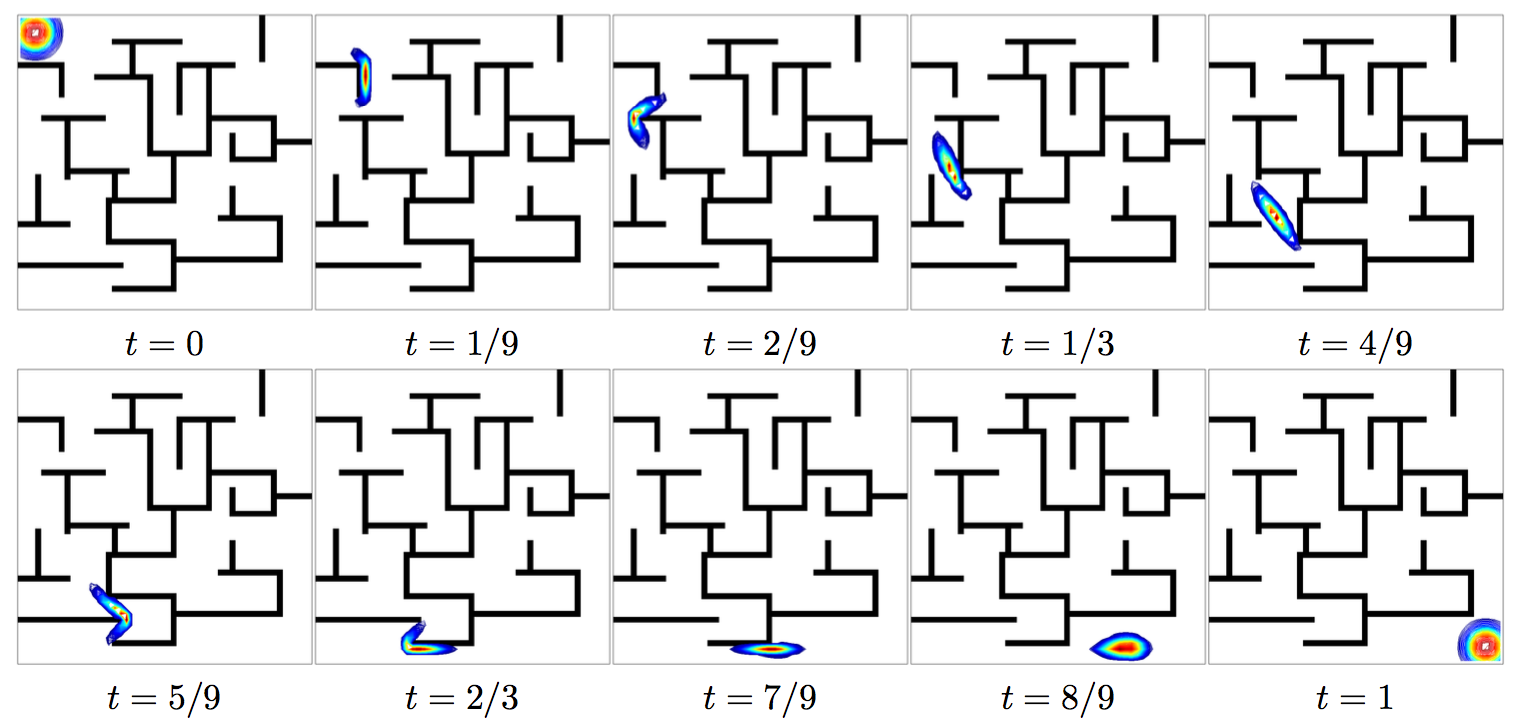
\includegraphics[width=\linewidth]{dynamic/dynamic-maze}
\caption{\label{fig-dynamic-maze}
Solution $\al_t$ of dynamic OT computed with a proximal splitting scheme.
}
\end{figure}



%%%%%%%%%%%%%%%%%%%%%%%%%%%%%%%%%%%%%%%%%
\section{Dynamical Unbalanced OT}
\label{dynamic-unbalanced}

In order to be able to match input measures with different mass $\al_0(\Xx) \neq \al_1(\Xx)$ (the so-called ``unbalanced'' settings, the terminology introduced by~\citet{benamou2003numerical}), and also to cope with local mass variation,
%
several normalizations or relaxations have been proposed, in particular by relaxing the fixed marginal constraint; see~\S\ref{sec-unbalanced}. 
A general methodology consists in introducing a source term $s_t(x)$ in the continuity equation~\eqref{eq-mass-conservation}. We thus consider 
\eq{
	\bar\BBConstr(\al_0,\al_1) \eqdef 
	\enscond{ (\al_t,\Moment_t,s_t) }{
		\pd{\al_t}{t} + \diverg(\Moment_t) = s_t, 
		\al_{t=0}=\al_0, 
		\al_{t=1}=\al_1
	}.
}
The crucial question is how to measure the cost associated to this source term and introduce it in the original dynamic formulation~\eqref{eq-bb-convex}. Several proposals appear in the literature, for instance, using an $L^2$ cost~\citet{piccoli2014generalized}.  
%
In order to avoid having to ``teleport'' mass (mass which travels at infinite speed and suddenly grows in a region where there was no mass before), the associated cost should be infinite. It turns out that this can be achieved in a simple convex way, by also allowing $s_t$ to be an arbitrary measure (\emph{e.g.} using a 1-homogeneous cost) by penalizing $s_t$ in the same way as the momentum $\Moment_t$, 
\eql{\label{eq-wfr-dynamic}
	\WFR^2(\al_0,\al_1) = \umin{ (\al_t,\Moment_t,s_t)_t  \in \bar\BBConstr(\al_0,\al_1)  }
		\Theta(\al,\Moment,s),
}
\eq{
	\qwhereq \Theta(\al,\Moment,s) \eqdef 
		\int_0^1 \int_{\RR^d} \pa{ 
			\theta(\al_t(x),\Moment_t(x)) + \tau \theta(\al_t(x),s_t(x)) 
		}\d x \d t,
}
where $\th$ is the convex 1-homogeneous function introduced in~\eqref{eq-theta-dynamic}, and $\tau$ is a weight controlling the trade-off between mass transportation and mass creation/destruction. This formulation was proposed independently by several authors~\citep{LieroMielkeSavareShort,2017-chizat-focm,kondratyev2015}. This ``dynamic'' formulation has a ``static'' counterpart; see Remark~\ref{rem-wfr-static}. 
%
The convex optimization problem~\eqref{eq-wfr-dynamic} can be solved using methods similar to those detailed in~\S\ref{sec-prox-solvers}. 
%
Figure~\ref{fig-unbalanced-dynamic} displays a comparison of several unbalanced OT dynamic interpolations.
%
This dynamic formulation resembles ``metamorphosis'' models for shape registration~\citep{Metamorphosis2005}, and a more precise connection is detailed in~\citep{maas2015generalized,maas2016generalized}. 

As $\tau \rightarrow 0$, and if $\al_0(\Xx) = \al_1(\Xx)$, then one retrieves the classical OT problem, $\WFR(\al_0,\al_1) \rightarrow \Wass(\al_0,\al_1)$. In contrast, as $\tau \rightarrow +\infty$, this distance approaches the Hellinger metric over densities
\begin{align*}
	\frac{1}{\tau}\WFR(\al_0,\al_1)^2\; \overset{\tau \rightarrow +\infty} \longrightarrow 
	&\int_{\Xx} | \sqrt{\density{\al_0}(x)} - \sqrt{\density{\al_1}(x)} |^2 \d x \\
	=& \int_{\Xx} | 1 - \sqrt{ \frac{\d\al_1}{\d\al_0}(x) } |^2 \d \al_0(x).
\end{align*}

\begin{figure}[h!]
\centering
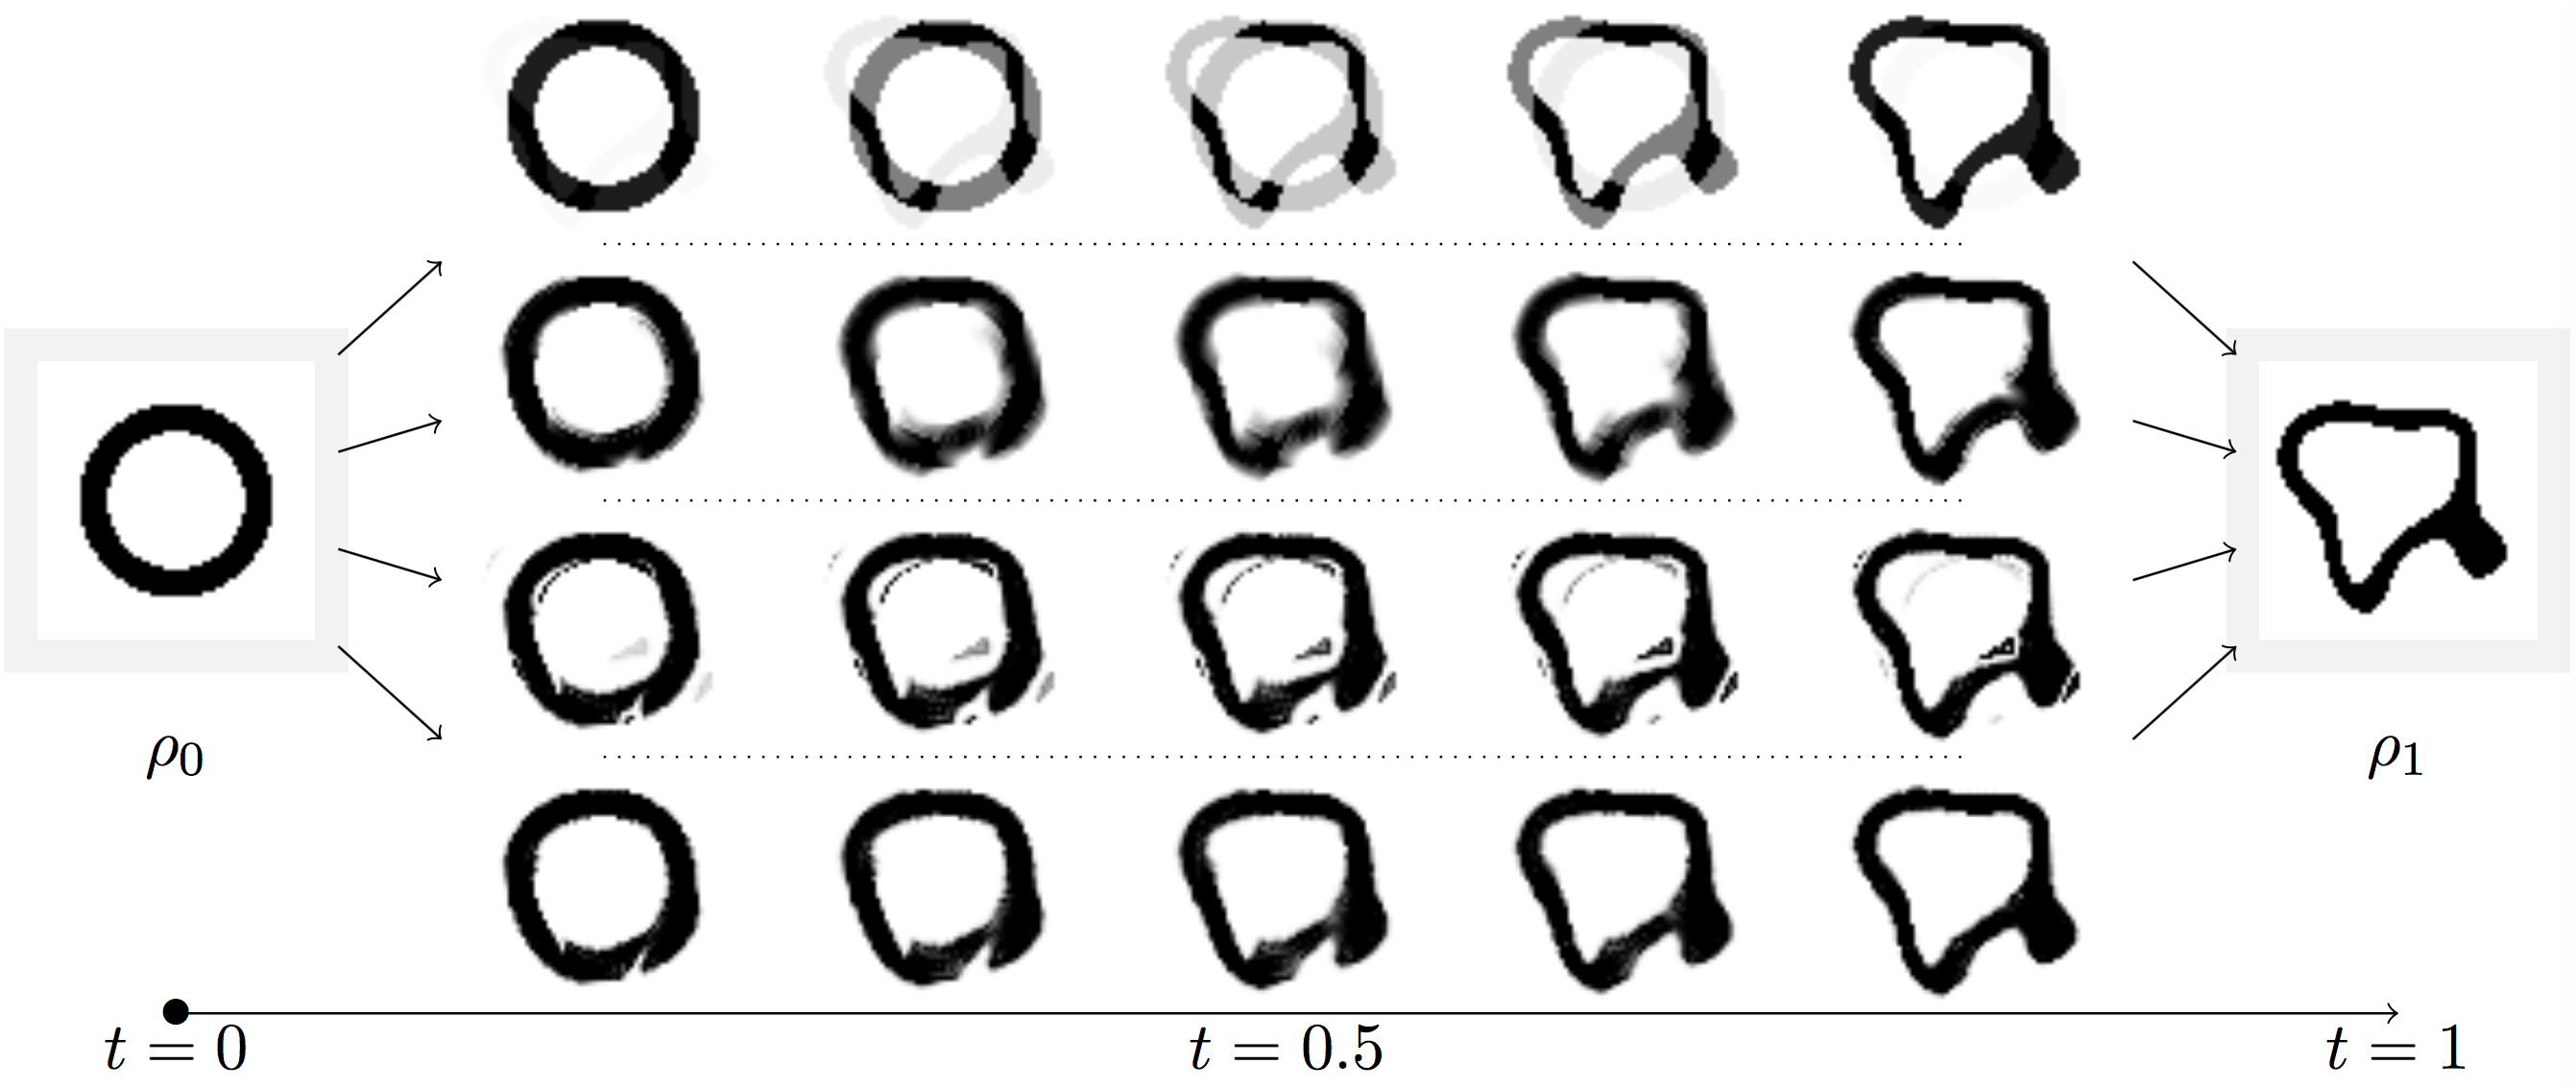
\includegraphics[width=\linewidth]{unbalanced/unbalanced-dynamic}
\caption{\label{fig-unbalanced-dynamic}
Comparison of Hellinger (first row), Wasserstein (row 2), partial optimal transport (row 3), and Wasserstein--Fisher--Rao (row 4) dynamic interpolations.
}
\end{figure}




%%%%%%%%%%%%%%%%%%%%%%%%%%%%%%%%%%%%%%%%%
\section{More General Mobility Functionals}
\label{eq-generic-modibility}

It is possible to generalize the dynamic formulation~\eqref{eq-bb-convex} by considering other ``mobility functions'' $\th$ in place of the one defined in~\eqref{eq-theta-dynamic}. A possible choice for this mobility functional is proposed in~\citet{dolbeault2009new},
\eql{\label{eq?generic-mobility}
	\foralls (a,b) \in \RR_+ \times \RR^\dim, \quad
	\th(a,b) = a^{s-p} \norm{b}^{p},
}
where the parameter should satisfy $p \geq 1$ and $s \in [1,p]$ in order for $\th$ to be convex. 
%
Note that this definition should be handled with care in the case $1<s\leq p$ because $\th$ does not have a linear growth at infinity, so that solutions to~\eqref{eq-bb-convex} must be constrained to have a density with respect to the Lebesgue measure. 

The case $s=1$ corresponds to the classical OT problem and the optimal value of~\eqref{eq-bb-convex} defines $\Wass_p(\al,\be)$. In this case, $\th$ is 1-homogeneous, so that solutions to~\eqref{eq-bb-convex} can be arbitrary measures. The case $(s=1,p=2)$ is the initial setup considered in~\eqref{eq-bb-convex} to define $\Wass_2$. 

The limiting case $s=p$ is also interesting, because it corresponds to a dual Sobolev norm $W^{-1,p}$ and the value of~\eqref{eq-bb-convex} is then equal to
\eq{
	\norm{\al-\be}_{W^{-1,p}(\RR^\dim)}^p = 
	\umin{\f} \enscond{ \int_{\RR^\dim} \f  \d(\al-\be)}{  \int_{\RR^\dim} \norm{ \nabla f(x) }^q \d x \leq 1 }
}
for $1/q+1/p=1$.
%
In the limit $(p=s,q) \rightarrow (1,\infty)$, one recovers the $\Wass_1$ norm.
%
The case $s=p=2$ corresponds to the Sobolev $H^{-1}(\RR^\dim)$ Hilbert norm defined in~\eqref{eq-dual-sobolev-div}.


\todoK{Speak of the connexion with geodesic in shape space~\citet{beg2005computing}. }

\todoK{``Here many computation techniques related to optimal control and Hamilton-Jacobi equations have not mentioned. The connections between optimal transport and Mean field games may be the other interesting direction. Many techniques developed in numerical optimal transport can be applied to general control problems in the set of probability space. For example, a new Hopf-Lax formula is introduced for dynamical optimal transport problem. See related discussions in~\citet{gangbo2008hamilton}.''}



%%%%%%%%%%%%%%%%%%%%%%%%%%%%%%%%%%%%%%%%%
\section{Dynamic Formulation over the Paths Space}
\label{sec-entropic-dynamic}

There is a natural dynamical formulation of both classical and entropic regularized (see~\S\ref{c-entropic}) formulations of OT, which is based on studying abstract optimization problems on the space $\bar\Xx$ of all possible paths $\ga : [0,1] \rightarrow \Xx$ (\ie curves) on the space $\Xx$. 
% 
For simplicity, we assume $\Xx=\RR^\dim$, but this extends to more general spaces such as geodesic spaces and graphs.
%
Informally, the dynamic of ``particles'' between two input measures $\al_0,\al_1$ at times $t=0,1$ is described by a probability distribution $\bar\pi \in \Mm_+^1(\bar\Xx)$. Such a distribution should satisfy that the distributions of starting and end points must match $(\al_0,\al_1)$, which is formally written using push-forward as
\eq{
	\bar\Couplings(\al_0,\al_1) \eqdef \enscond{ \bar\pi \in \Mm_+^1(\bar\Xx) }{ \bar P_{0\sharp} \bar\pi = \al_0, \bar P_{1\sharp} \bar\pi = \al_1  },
}
where, for any path $\ga \in \bar\Xx$, $P_0(\ga) = \ga(0), P_1(\ga) = \ga(1)$.

%%%%
\paragraph{OT over the space of paths.}

The dynamical version of classical OT~\eqref{eq-mk-generic}, formulated over the space of paths, then reads
\eql{\label{eq-ot-pathsspace}
	\Wass_2(\al_0,\al_1)^2 =
	\umin{ \bar\pi \in \bar\Couplings(\al_0,\al_1) } \int_{\bar\Xx} \Ll(\ga)^2 \d\bar\pi(\ga),
}
where $\Ll(\ga) = \int_0^1 |\ga'(s)|^2 \d s$ is the kinetic energy of a path $s \in [0,1] \mapsto \ga(s) \in \Xx$. The connection between optimal couplings $\pi^\star$ and $\bar\pi^\star$ solving respectively~\eqref{eq-ot-pathsspace} and~\eqref{eq-mk-generic} is that $\bar\pi^\star$ only gives mass to geodesics joining pairs of points in proportion prescribed by $\pi^\star$. In the particular case of discrete measures, this means that 
\eq{
	\pi^\star = \sum_{i,j} \P_{i,j} \de_{(x_i,y_j)}
	\qandq
	\bar\pi^\star = \sum_{i,j} \P_{i,j} \de_{\ga_{x_i,y_j}},
} 
where $\ga_{x_i,y_j}$ is the geodesic between $x_i$ and $y_j$. Furthermore, the measures defined by the distribution of the curve points $\ga(t)$ at time $t$, where $\ga$ is drawn following $\bar\pi^\star$, \ie
\eql{\label{eq-interpolation-spacepaths}
	 t \in [0,1] \mapsto \al_t \eqdef P_{t\sharp} \bar\pi^\star 
	 \qwhereq
	 P_t(\ga) = \ga(t) \in \Xx,  
}
is a solution to the dynamical formulation~\eqref{eq-bb-convex}, \ie it is the displacement interpolation. 
%
In the discrete case, one recovers~\eqref{eq-mccann-discrete}. 

%%%%
\paragraph{Entropic OT over the space of paths.}

We now turn to the re-interpretation of entropic OT, defined in Chapter~\ref{c-entropic}, using the space of paths. 
%
Similarly to~\eqref{eq-entropic-generic-proj}, this is defined using a Kullback--Leibler projection, but this time of a reference measure over the space of paths $\bar\Kk$ which is the distribution of a reversible Brownian motion (Wiener process), which has a uniform distribution at the initial and final times
\eql{\label{eq-shrodinger-paths}
	\umin{ \bar\pi \in \bar\Couplings(\al_0,\al_1) } \KL(\bar\pi|\bar\Kk).
}
We refer to the review paper by~\citet{LeonardSchroedinger} for an overview of this problem and an historical account of the work of~\citet{Schroedinger31}. 
%
One can show that the (unique) solution $\bar\pi_\varepsilon^\star$ to~\eqref{eq-shrodinger-paths} converges to a solution of~\eqref{eq-ot-pathsspace} as $\varepsilon \rightarrow 0$. Furthermore, this solution is linked to the solution of the static entropic OT problem~\eqref{eq-entropic-generic} using Brownian bridge $\bar\ga_{x,y}^\varepsilon \in \bar\Xx$ (which are similar to fuzzy geodesic and converge to $\de_{\ga_{x,y}}$ as $\varepsilon \rightarrow 0$). In the discrete setting, this means that 
\eql{\label{eq-brownian-bridge-interp}
	\pi_\varepsilon^\star = \sum_{i,j} \P_{\varepsilon,i,j}^\star \de_{(x_i,y_j)}
	\qandq
	\bar\pi_\varepsilon^\star = \sum_{i,j} \P_{\varepsilon,i,j}^\star \bar\ga_{x_i,y_j}^\varepsilon,
}
where $\P_{\varepsilon,i,j}^\star$ can be computed using Sinkhorn's algorithm. 
%
Similarly to~\eqref{eq-interpolation-spacepaths}, one then can define an entropic interpolation as 
\eq{
	\al_{\varepsilon,t} \eqdef \P_{t\sharp} \bar\pi_\varepsilon^\star. 
}
Since the law $\P_{t\sharp} \bar\ga_{x,y}^\varepsilon$ of the position at time $t$ along a Brownian bridge is a Gaussian $\Gg_{t(1-t)\varepsilon^2}(\cdot-\ga_{x,y}(t))$ of variance $t(1-t)\varepsilon^2$ centered at $\ga_{x,y}(t)$, one can deduce that $\al_{\varepsilon,t}$ is a Gaussian blurring of a set of traveling Diracs
\eq{
	\al_{\varepsilon,t} =
	\sum_{i,j} \P_{\varepsilon,i,j}^\star \Gg_{t(1-t)\varepsilon^2}( \cdot - \ga_{x_i,y_j}(t) ). 
}
The resulting mixture of Brownian bridges is displayed on Figure~\ref{fig-schrodinger-dynamic}.


% G B D H
\newcommand{\MyFigSchrDyn}[1]{\includegraphics[width=.245\linewidth,trim=50 45 38 35,clip]{schrodinger-dynamic/schrodinger-dynamic-eps#1}}
%%% FIG %%%
\begin{figure}[h!]\centering
\centering
\begin{tabular}{@{}c@{}c@{}c@{}c@{}}
\MyFigSchrDyn{5}&
\MyFigSchrDyn{50}&
\MyFigSchrDyn{200}&
\MyFigSchrDyn{1000}\\
$\varepsilon=0$ & $\varepsilon=.05$ & $\varepsilon=0.2$ & $\varepsilon=1$
\end{tabular}
%%%
\caption{%%%
Samples from Brownian bridge paths associated to the Schr\"odinger entropic interpolation~\eqref{eq-brownian-bridge-interp} over path space. Blue corresponds to $t=0$ and red to $t=1$. 
} \label{fig-schrodinger-dynamic}
\end{figure}
%%% FIG %%%

Another way to describe this entropic interpolation $(\al_t)_t$ is using a regularization of the Benamou--Brenier dynamic formulation~\eqref{eq-bb-non-cvx}, namely \todoK{check how $\varepsilon$ enters the picture}
\eql{\label{eq-bb-non-cvx-entropy}
	\umin{ (\al_t,\speed_t)_t \text{ sat. \eqref{eq-cons-bb-ncvx}} }
		\int_0^1 \int_{\RR^d}  \pa{
			 \norm{\speed_t(x)}^2  + \frac{\varepsilon}{4} \norm{ \nabla \log(\al_t)(x) }^2
			 } 
			 \d\al_t(x) \d t; 
}
see~\citep{gentil2015analogy,chen2016relation}.




